\chapter{Document contenu dans plusieurs fichiers}
\label{chap:include}

Un document {\LaTeX} comporte toujours un préambule suivi du corps du
texte. Lorsque ceux-ci sont relativement courts (peu de commandes
spéciales et moins d'une vingtaine de pages de texte), il demeure
assez simple et convivial d'en faire l'édition dans un seul fichier à
l'aide de son éditeur de texte favori.

Cependant, si le préambule devient long et complexe ou, surtout,
lorsque l'ampleur du document augmente jusqu'à compter un grand nombre
de pages sur plusieurs chapitres, il convient de répartir les divers
éléments du document dans des fichiers séparés.

La segmentation en plusieurs fichiers rend l'édition du texte plus
simple et plus efficace. De plus, durant la phase de rédaction, elle
peut significativement accélérer, la compilation des documents très
longs ou comptant plusieurs images.


\section{Insertion de contenu avec la commande \cs{input}}
\label{sec:include:input}

La commande \cmd{\input} permet d'insérer le contenu d'un autre
fichier dans un document {\LaTeX}. La syntaxe de la commande est
\begin{lstlisting}
\input`\marg{fichier}'
\end{lstlisting}
où le nom du fichier à insérer est \meta{fichier}\code{.tex}. On
laisse donc tomber l'extension \code{.tex}, qui est implicite. Le
contenu du fichier est inséré tel quel dans le document, comme s'il
avait été tapé dans le fichier qui contient l'appel à \cmd{\input}.

Le procédé est surtout utile pour sauvegarder séparément des bouts de
code qui pourraient nuire à l'édition du texte (figures, longs
tableaux) ou qui sont communs entre plusieurs documents (licence
d'utilisation, auteur et affiliation).

La commande peut aussi être utilisée dans le préambule pour charger
une partie ou l'ensemble de celui-ci. Cela permet de composer un même
préambule pour plusieurs documents. Il suffit alors de faire
d'éventuelles modifications à un seul endroit pour les voir prendre
effet dans tous les documents.


\section{Insertion de parties avec la commande \cs{include}}
\label{sec:include:include}

Extrait de la %
\doc{ulthese}{http://texdoc.net/pkg/ulthese/} %
de la classe \class{ulthese}:
\begin{quote}
  «Il est recommandé de segmenter tout document d'une certaine ampleur
  dans des fichiers \verb=.tex= distincts pour chaque partie ---
  habituellement un fichier par chapitre. Le document complet est
  composé à l'aide d'un fichier maître qui contient le préambule
  {\LaTeX} et un ensemble de commandes \verb=\include= pour réunir les
  parties dans un tout.»
\end{quote}

Comme \cmd{\input}, la commande \cmd{\include} insère le contenu
d'un autre fichier dans un document {\LaTeX}. Son effet est cependant
différent et c'est son utilisation qui permet d'accélérer la
compilation d'un long document.

L'insertion d'un fichier avec \cmd{\include} débute toujours une
nouvelle page. On utilisera donc \cmd{\include} principalement pour
insérer des chapitres entiers plutôt que seulement des portions de
texte. De plus, un fichier inséré avec \cmd{\include} peut contenir
des appels à \cmd{\input}, mais pas à \cmd{\include}.

La syntaxe de la commande \cmd{\include} est
\begin{lstlisting}
\include`\marg{fichier}'
\end{lstlisting}
où le nom du fichier à insérer est \meta{fichier}\code{.tex}. Ici
aussi on laisse tomber l'extension \code{.tex} qui est implicite.

 La structure type d'un fichier maître est la suivante:
\begin{lstlisting}
\documentclass{ulthese}
  [...]

\begin{document}

\frontmatter

%%% Copyright (C) 2018 Vincent Goulet
%%%
%%% Ce fichier fait partie du projet
%%% «Rédaction avec LaTeX»
%%% http://github.com/vigou3/formation-latex-ul
%%%
%%% Cette création est mise à disposition selon le contrat
%%% Attribution-Partage dans les mêmes conditions 4.0
%%% International de Creative Commons.
%%% http://creativecommons.org/licenses/by-sa/4.0/

\chapter{Introduction}
\label{chap:introduction}

Le présent ouvrage tire son origine d'une formation sur la rédaction
de thèses et de mémoires avec {\LaTeX} développée pour la Bibliothèque
de l'Université Laval. La formation aborde les concepts de base pour
un nouvel utilisateur: processus d'édition, compilation,
visualisation; séparation du contenu et de l'apparence du texte; mise
en forme du texte; séparation du document en parties; rudiments du
mode mathématique. Transformée en prose, la série de diapositives qui
appuie la présentation correspond grosso modo aux quatre premiers
chapitres de l'ouvrage.

Les six autres chapitres visent à rendre l'utilisateur de {\LaTeX}
débutant ou intermédiaire autonome dans la rédaction de documents
relativement complexes comportant des tableaux, des figures, des
équations mathématiques élaborées, une bibliographie, etc. Nous avons
aussi émaillé le texte de conseils et d'astuces glanés au fil de nos
vingt années d'utilisation du système de mise en page.

Les nombreuses références à la classe de documents \class{ulthese}
s'adressent au premier public de l'ouvrage: les étudiantes et
étudiants de l'Université Laval occupés à la rédaction de leur thèse
ou de leur mémoire. Ils devront utiliser cette classe pour composer un
document conforme aux règles générales de présentation matérielle de
la Faculté des études supérieures et postdoctorales. Les autres
lecteurs pourront sans mal escamoter ces passages.

Chaque chapitre comporte quelques exercices. Les solutions se trouvent
en annexe. En consultation électronique, le numéro d'un exercice est,
le cas échéant, un hyperlien vers sa solution, et vice versa.

Un index en fin d'ouvrage collige les références aux commandes et
environnements {\LaTeX}, ainsi qu'aux noms de paquetages et de
classes.

\subsection*{Autres références utiles}

L'ouvrage n'a aucune prétention d'exhaustivité. La consultation de
documentation additionnelle pourra s'avérer nécessaire pour réaliser
des mises en page plus élaborées. À cet égard, nous recommandons
chaudement le livre de \citet{Kopka:latex:4e} --- il a servi
d'inspiration pour ce document à maints endroits. La très complète
documentation (plus de 600~pages!) de la classe \class{memoir}
\citep{memoir} constitue une autre référence de choix. Nous
recommandons également:
\begin{itemize}
\item \link{http://fr.wikibooks.org/wiki/LaTeX}{\emph{LaTeX} dans
    Wikilivre} pour de la documentation en ligne, en français et
  libre;
\item le très actif forum de discussion
  \link{http://tex.stackexchange.com}{{\TeX}--{\LaTeX} Stack Exchange}
  (avant de penser y poser une question, vérifier que la réponse ne se trouve
  pas déjà dans le forum\dots\ ce qui risque fort d'être le cas);
\item la très complète
  \link{http://www.tex.ac.uk/cgi-bin/texfaq2html}{%
    \emph{foire aux questions}} (en anglais) du groupe des
  utilisateurs de {\LaTeX} du Royaume-Uni.
\end{itemize}

\subsection*{Installation d'une distribution}

L'utilisation de {\LaTeX} requiert évidemment une distribution du
système. Nous recommandons la distribution {\TeX}~Live administrée par
le {\TeX} Users Group. Les hyperliens ci-dessous mènent vers des
vidéos qui expliquent comment installer cette distribution.
\begin{itemize}
\item \capsule{https://youtu.be/kA53EQ3Q47w}{%
    Installation sur macOS}
\item \capsule{https://youtu.be/7MfodhaghUk}{%
    Installation sur Windows}
\end{itemize}

\subsection*{Hyperliens vers la documentation}

Le texte comporte plusieurs renvois vers la documentation d'un
paquetage ou d'une classe, par exemple vers la %
\doc{memoir}{http://texdoc.net/pkg/memoir/} %
de la classe \class{memoir}. L'hyperlien mène vers la version en ligne
de la documentation dans le site %
\link{http://texdoc.net}{TeXdoc Online}. On trouve également dans la
marge le nom du fichier correspondant (sans l'extension \code{.pdf})
sur un système doté de {\TeX}~Live.

La plupart des logiciels intégrés de rédaction {\LaTeX} offrent une
interface pour accéder à cette documentation.
\begin{itemize}
\item TeXShop: menu \code{Aide|Afficher l'aide pour le
    package} (\optkey\,\cmdkey\, I).
\item Texmaker: menu \code{Aide|TeXDoc [selection]}.
\item GNU~Emacs: commande \code{TeX-doc} (\code{C-c ?}) du mode
  spécialisé AUC{\TeX}.
\end{itemize}
Le lecteur devrait consulter la rubrique d'aide de son éditeur pour
savoir s'il offre une interface au système de gestion de la
documentation Texdoc de {\TeX}~Live.

\subsection*{Fichiers d'accompagnement}

Ce document devrait être accompagné des fichiers nécessaires pour
compléter certains exercices figurant à la fin des chapitres, ainsi
que d'un gabarit \fichier{exercice\_gabarit.tex} pour composer les
solutions des autres exercices. Si ce n'est pas le cas, récupérer les
fichiers dans le site \link{\ctanurl}{\emph{Comprehensive TeX Archive
    Network} (CTAN)}.

%%% Local Variables:
%%% mode: latex
%%% TeX-master: "formation-latex-ul"
%%% TeX-engine: xetex
%%% encoding: utf-8
%%% End:

\tableofcontents*

\mainmatter
\include{historique}            % premier chapitre
\include{modele}                % deuxième chapitre
[...]

\end{document}
\end{lstlisting}

Le principal avantage de \cmd{\include} par rapport à \cmd{\input}
réside dans le fait que {\LaTeX} peut préserver entre les compilations
les informations telles que les numéros de pages, de sections ou
d'équations, ainsi que les références. Cela permet, par exemple, de
compiler le texte d'un seul chapitre --- plutôt que le document entier
--- et néanmoins obtenir une image représentative du chapitre.
Procéder ainsi accélère significativement la compilation des documents
longs ou complexes.

La commande \cmd{\includeonly}, que l'on utilise exclusivement dans le
préambule, sert à spécifier le ou les fichiers à compiler tout en
préservant la numérotation et les références. Sa syntaxe est
\begin{lstlisting}
\includeonly`\marg{liste\_fichiers}'
\end{lstlisting}
où \meta{liste\_fichiers} contient les noms des fichiers à
inclure dans la compilation, séparés par des virgules et sans
l'extension \code{.tex}.

Lors de l'utilisation de la commande \cmd{\includeonly}, toute la
numérotation dans les fichiers \meta{liste\_fichiers} suivra celle
établie lors de la compilation précédente. Si l'édition des fichiers
de \meta{liste\_fichiers} cause des changements dans la numérotation
et les références dans les autres parties du document, une nouvelle
compilation de l'ensemble ou d'une partie de celui-ci s'avérera
nécessaire.

\begin{exemple}
  Un document est composé en plusieurs parties avec les commandes
  suivantes:
\begin{lstlisting}
\include{chapitre1.tex}
\include{chapitre2.tex}
\include{chapitre3.tex}
\end{lstlisting}
  Les chapitres débutent respectivement aux pages~1, 23 et 41.
  \begin{itemize}
  \item Si on ajoute au préambule du document la commande
\begin{lstlisting}
\includeonly{chapitre2}
\end{lstlisting}
    le numéro du chapitre sera toujours 2 et le folio de
    la première page sera toujours 23, même si les 22 pages
    précédentes ne se trouvent pas dans le document.
  \item Si l'on modifie le fichier \code{chapitre2} de telle sorte que
    le chapitre se termine maintenant à la page 46, il faudra
    recompiler le document avec au moins les fichiers \code{chapitre2}
    et \code{chapitre3} pour que les pages du chapitre~3 soient
    renumérotées à partir de 47.
  \end{itemize}
  \qed
\end{exemple}

L'\autoref{ex:include} illustre mieux le cycle typique
d'utilisation des commandes \cmd{\include} et \cmd{\includeonly}.



%%%
%%% Exercices
%%%

\section{Exercices}
\label{sec:include:exercices}

\begin{exercice}[nosol]
  \label{ex:include}
  Cet exercice fait appel au fichier maître
  \fichier{exercice\_include.tex} et à plusieurs fichiers auxiliaires.
  Schématiquement, le document est composé ainsi:

  \medskip
  \begin{minipage}{\linewidth}
    \dirtree{%
      .1 exercice\_include.tex.
      .2 {\textbackslash}input pagetitre.tex.
      .2 {\textbackslash}include presentation.tex.
      .3 {\textbackslash}includegraphics console-screenshot.pdf.
      .2 {\textbackslash}include emacs.tex.
    }
  \end{minipage}
  \medskip

  La commande \cmd{\includegraphics} permet d'insérer une image dans
  un document {\LaTeX}. Elle provient du paquetage \pkg{graphicx}.

  \begin{enumerate}
  \item Étudier le code source du fichier maître
    \fichier{exercice\_include.tex}, puis le compiler deux à trois
    fois jusqu'à ce que toutes les références internes soient à jour.
    Il est normal à ce stade que la figure~1 du document soit vide.
  \item Ajouter dans le préambule du fichier maître la commande
\begin{lstlisting}
\includeonly{emacs}
\end{lstlisting}
    puis compiler le document.

    Observer que, malgré l'absence du chapitre~1, la numérotation et
    les références demeurent à jour, notamment la table des matières.
  \item Remplacer la commande ajoutée en b) dans le préambule du
    fichier maître par la commande
\begin{lstlisting}
\includeonly{presentation}
\end{lstlisting}
    Vers la fin du fichier \fichier{presentation.tex}, activer la
    commande
\begin{lstlisting}
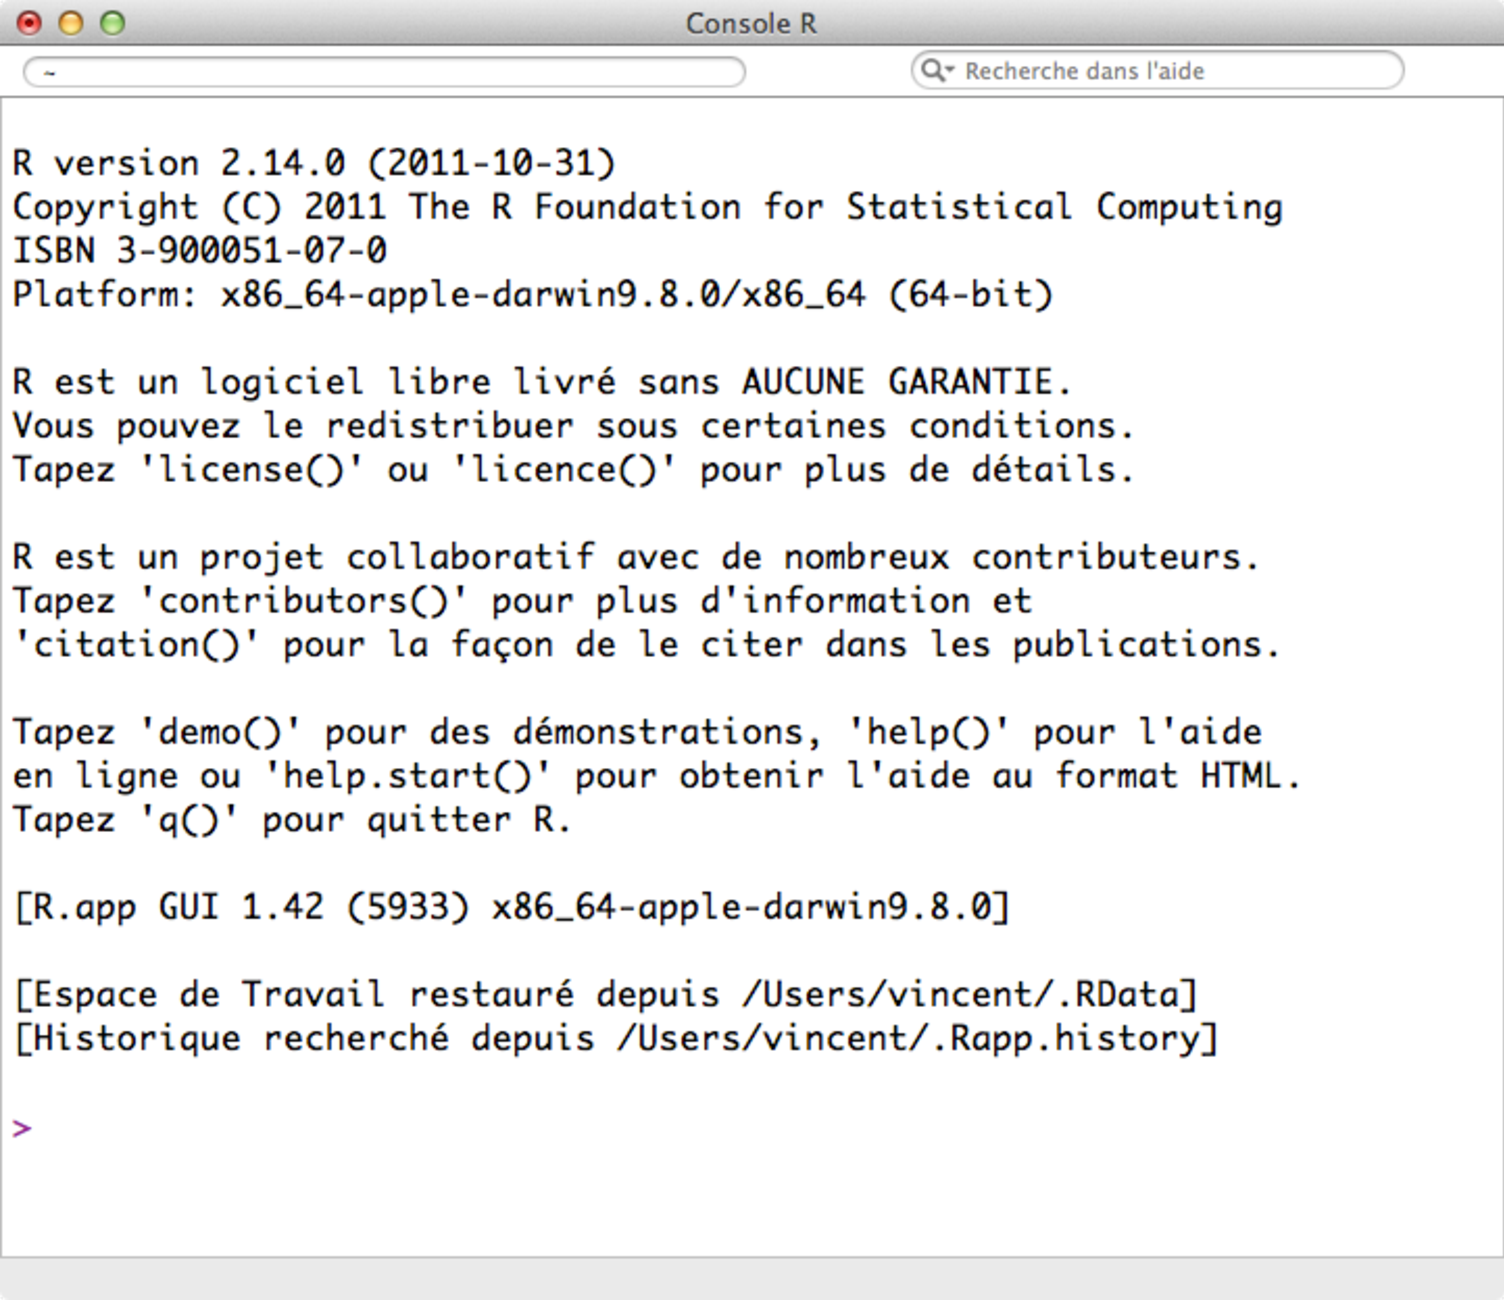
\includegraphics[width=\textwidth]{console-screenshot}
\end{lstlisting}
    en supprimant le symbole \% au début de la ligne. Compiler de
    nouveau le document deux fois.

    Les modifications ont eu pour effet d'ajouter une page au
    chapitre~1. Observer que selon la table des matières, le
    chapitre~2 débute toujours à la page~3 alors que celle-ci est
    maintenant occupée par la figure~1.
  \item Afin de corriger la table des matières, désactiver dans le
    préambule du fichier maître la commande \cmd{\includeonly}, puis
    compiler de nouveau le document quelques fois.
  \end{enumerate}
\end{exercice}

\begin{exercice}[nosol]
  Déplacer dans un fichier \fichier{preambule.tex} toutes les lignes
  du préambule du fichier \fichier{exercice\_include.tex} utilisé à
  l'exercice précédent, à l'exception de celles relatives à la page
  titre (titre, auteur, date). Insérer le préambule dans
  \fichier{exercice\_include.tex} avec la commande \cmd{\input}.
\end{exercice}

%%% Local Variables:
%%% mode: latex
%%% TeX-engine: xetex
%%% TeX-master: "formation_latex-partie_2"
%%% coding: utf-8
%%% End:
